\chapter{PC Software}
\section{Software flow}
 This code creates a GUI that on the front end provides the user with the control of load LED PWM and control over the charging of the battery. The user is also provided with numerical data and visual data  on the battery current \& voltage, supply voltage and LDR readings. The user will also be able to save this visual data to a csv file. The application backend is operated through serial communication between the beetle and the PC.
\begin{figure}[!htb]
	\centering
	\includegraphics[width=0.73\linewidth]{Figures/A9/A9.png	}
	\caption{PC Software flow diagram}
	\label{fig:flow}
\end{figure}



The given code was used as a base for the developed application\cite{}. 
\section{Functions Overview}
\subsection{Functions inside loop}
\subsection{Button Functions}



\begin{figure}[!htb]
	\centering
	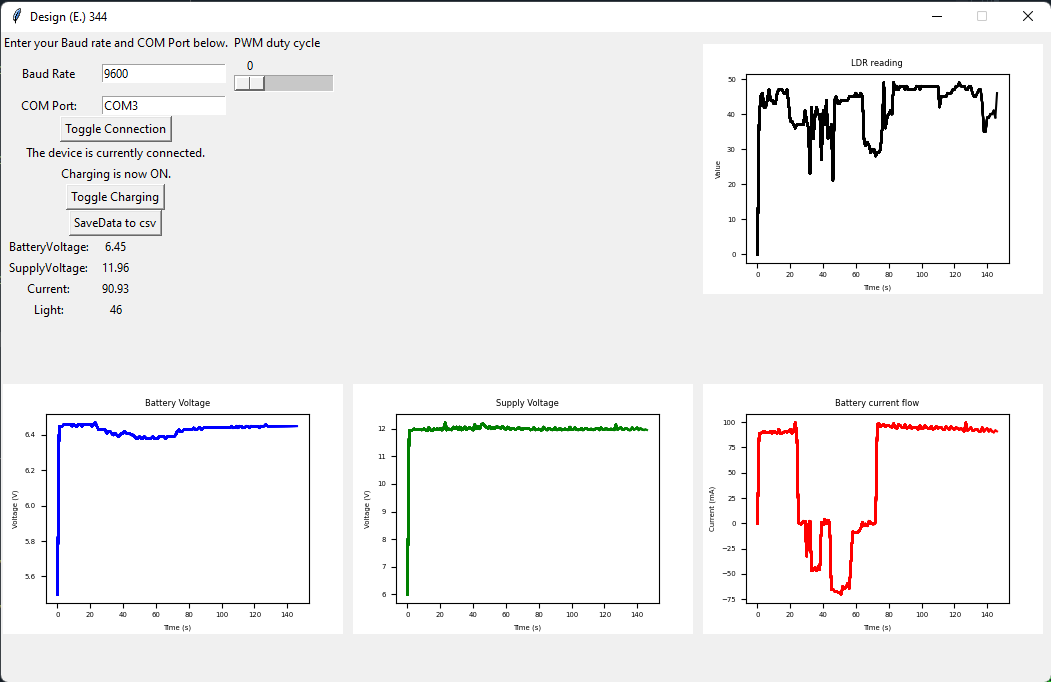
\includegraphics[width=1\linewidth]{Figures/A9/GUI.png}
	\caption{Software GUI}
	\label{fig:flow}
\end{figure}